 	\documentclass{llncs}
%%%%%%%%%%%%%%%%%%%%%%%%%%%%%%%%%%%%%%%%%%%%%%%%%%%%%%%%%%%
%% package sillabazione italiana e uso lettere accentate
\usepackage[utf8]{inputenc}\usepackage[T1]{fontenc}
%%%%%%%%%%%%%%%%%%%%%%%%%%%%%%%%%%%%%%%%%%%%%%%%%%%%%%%%%%%%%

\usepackage{url}
\usepackage{xspace}
\usepackage{hyperref}

\usepackage[a4paper,hmargin=4.4cm, vmargin=5.2cm]{geometry}
\makeatletter
%%%%%%%%%%%%%%%%%%%%%%%%%%%%%% User specified LaTeX commands.
\usepackage{manifest}

\makeatother

\usepackage{listings}
\usepackage{xcolor}


\usepackage{inconsolata}

\usepackage{color}

\definecolor{pblue}{rgb}{0.13,0.13,1}
\definecolor{pgreen}{rgb}{0,0.5,0}
\definecolor{pred}{rgb}{0.9,0,0}
\definecolor{pgrey}{rgb}{0.46,0.45,0.48}

\usepackage{listings}
\lstset{language=Java,
  showspaces=false,
  showtabs=false,
  breaklines=true,
  showstringspaces=false,
  breakatwhitespace=true,
  commentstyle=\color{pgreen},
  keywordstyle=\color{pblue},
  stringstyle=\color{pred},
  basicstyle=\ttfamily,
  moredelim=[il][\textcolor{pgrey}]{\$\$},
  moredelim=[is][\textcolor{pgrey}]{\%\%}{\%\%},  
   linewidth=14cm,
	frame=single,
    basicstyle=\footnotesize, %or \small or \footnotesize et
   numberstyle=\footnotesize,
   numbersep=9pt,
   tabsize=2,
   breaklines=true,
   showtabs=false,
   captionpos=b
}


%%%%%%%
 \newif\ifpdf
 \ifx\pdfoutput\undefined
 \pdffalse % we are not running PDFLaTeX
 \else
 \pdfoutput=1 % we are running PDFLaTeX
 \pdftrue
 \fi
%%%%%%%
 \ifpdf
 \usepackage[pdftex]{graphicx}
 \else
 \usepackage{graphicx}
 \fi
%%%%%%%%%%%%%%%
 \ifpdf
 \DeclareGraphicsExtensions{.pdf, .jpg, .tif}
 \else
 \DeclareGraphicsExtensions{.eps, .jpg}
 \fi
%%%%%%%%%%%%%%%
\usepackage{amsmath}
\usepackage{rotating}

\newenvironment{nscenter}
 {\parskip=0pt\par\nopagebreak\centering}
 {\par\noindent\ignorespacesafterend}

\newcommand{\java}{\textsf{Java}}
\newcommand{\contact}{\emph{Contact}}
\newcommand{\corecl}{\texttt{corecl}}
\newcommand{\medcl}{\texttt{medcl}}
\newcommand{\msgcl}{\texttt{msgcl}}
\newcommand{\android}{\texttt{Android}}
\newcommand{\dsl}{\texttt{DSL}}
\newcommand{\jazz}{\texttt{Jazz}}
\newcommand{\rtc}{\texttt{RTC}}
\newcommand{\ide}{\texttt{Contact-ide}}
\newcommand{\xtext}{\texttt{XText}}
\newcommand{\xpand}{\texttt{Xpand}}
\newcommand{\xtend}{\texttt{Xtend}}
\newcommand{\pojo}{\texttt{POJO}}
\newcommand{\junit}{\texttt{JUnit}}

\newcommand{\action}[1]{\texttt{#1}\xspace}
\newcommand{\code}[1]{{\small{\texttt{#1}}}\xspace}
\newcommand{\codescript}[1]{{\scriptsize{\texttt{#1}}}\xspace}

% Cross-referencing
\newcommand{\labelsec}[1]{\label{sec:#1}}
\newcommand{\xs}[1]{\sectionname~\ref{sec:#1}}
\newcommand{\xsp}[1]{\sectionname~\ref{sec:#1} \onpagename~\pageref{sec:#1}}
\newcommand{\labelssec}[1]{\label{ssec:#1}}
\newcommand{\xss}[1]{\subsectionname~\ref{ssec:#1}}
\newcommand{\xssp}[1]{\subsectionname~\ref{ssec:#1} \onpagename~\pageref{ssec:#1}}
\newcommand{\labelsssec}[1]{\label{sssec:#1}}
\newcommand{\xsss}[1]{\subsectionname~\ref{sssec:#1}}
\newcommand{\xsssp}[1]{\subsectionname~\ref{sssec:#1} \onpagename~\pageref{sssec:#1}}
\newcommand{\labelfig}[1]{\label{fig:#1}}
\newcommand{\xf}[1]{\figurename~\ref{fig:#1}}
\newcommand{\xfp}[1]{\figurename~\ref{fig:#1} \onpagename~\pageref{fig:#1}}
\newcommand{\labeltab}[1]{\label{tab:#1}}
\newcommand{\xt}[1]{\tablename~\ref{tab:#1}}
\newcommand{\xtp}[1]{\tablename~\ref{tab:#1} \onpagename~\pageref{tab:#1}}
% Category Names
\newcommand{\sectionname}{Section}
\newcommand{\subsectionname}{Subsection}
\newcommand{\sectionsname}{Sections}
\newcommand{\subsectionsname}{Subsections}
\newcommand{\secname}{\sectionname}
\newcommand{\ssecname}{\subsectionname}
\newcommand{\secsname}{\sectionsname}
\newcommand{\ssecsname}{\subsectionsname}
\newcommand{\onpagename}{on page}

\newcommand{\xauthA}{Stefano Belli}
\newcommand{\xfaculty}{II Faculty of Engineering}
\newcommand{\xunibo}{Alma Mater Studiorum -- University of Bologna}
\newcommand{\xaddrBO}{viale Risorgimento 2}
\newcommand{\xaddrCE}{via Venezia 52}
\newcommand{\xcityBO}{40136 Bologna, Italy}
\newcommand{\xcityCE}{47023 Cesena, Italy}

%
% Comments
%
%%% \newcommand{\todo}[1]{\bf{TODO:}\emph{#1}}


\begin{document}

\title{Dwarfort\\
 Relazione di progetto per Sistemi Autonomi}

%%% \author{\xauthA,\xauthB and \xauthC}
\author{\xauthA}

\institute{
  \xunibo\\\xaddrCE, \xcityCE\\\email{stefano.belli4\@studio.unibo.it}
}

\maketitle

%% \begin{abstract}
%% \footnotesize
%%This a Latex template to be used for the reports of Software Engineering.
%%\keywords{Software engineering, managed software development, reports, ....}
%%\end{abstract}



%%% \sloppy

%===========================================================================
\section{Introduzione}
\labelsec{Introduzione}
Lo scopo di questo progetto è quello di dimostrare e implementare alcuni dei concetti chiave della programmazione BDI presentati durante il corso di \textit{Sistemi Autonomi} presieduto dal prof. Andrea Omicini.\\
%È bene ricordare che, nei sistemi autonomi, gli agenti vengono interpretati come entità in grado di agire autonomamente all'interno dell'ambiente in cui vengono situati, adattando il loro comportamento e le loro azioni in base alla percezione del contesto in cui operano.\\
Più specificatamente, verrà approfondito il concetto di autonomia all'interno di un MAS attraverso la simulazione di una piccola società di agenti autonomi (nani) all'interno di un contesto (una miniera).\\
Come caso di studio questo progetto può avere una certa rilevanza perché integra concetti di collaborazione tra agenti, percezione dell'ambiente e deliberazione di processi atti a raggiungere obiettivi entro una serie di regole predefinite.
%===========================================================================

%===========================================================================
\newpage
\section{Requisiti}
Una miniera composta da diverse unità di scavatori, trasportatori e forgiatori deve riuscire a massimizzare l'estrazione delle risorse presenti in loco collaborando attivamente.\\
Nello specifico, ogni unità ha un preciso compito che dipende dalla sua mansione e posizione:
\begin{itemize}
\item I minatori, da qui in avanti chiamati \textit{miners}, dovranno rilevare tutte le vene di materiale presente nella loro cava personale e procedere alla loro estrazione.\\
Tutto il materiale estratto dovrà essere trasportato manualmente dalla vena di materiale al magazzino locale (\textit{storage}) restando entro i propri limiti di trasporto: un minatore non potrà mai infatti trasportare più kg di materiale di quanto la sua forza personale permetta.\\
La tipologia di materiale da estrarre (che può essere di ORO o FERRO) dipende unicamente dalla commessa comandata del nano forgiatore al momento.\\Infine, ogni \textit{miner} possiede un certo livello di tolleranza alla sete, che aumenta ad ogni operazione di scavo compiuta; arrivato al un livello critico di sete percepita, il minatore si fermerà finché non si sarà dissetato.\\
Essendo un nano, l'unica modo per dissetarsi è bere una birra.\\
\item I trasportatori, da qui in avanti chiamati \textit{carriers}, dovranno muovere il materiale stoccato nei magazzini locali delle miniere alla cava principale di controllo.\\Come per i \textit{miners}, la tipologia di minerale da trasportare verrà decisa unicamente dal \textit{forger} in base alle necessità del momento.\\
Per questioni logistiche, soltanto un \textit{carrier} alla volta potrà occupare una cave, e la scelta della destinazione dipenderà unicamente da loro (in altre parole, i nani trasportatori dovranno sapere orientarsi nella miniera e organizzarsi).\\
Qualora un \textit{miner} ne senta il bisogno, l'acquisizione di birra dal \textit{forger} ha la massima priorità: in tal caso infatti il \textit{carrier} abbandonerà ogni suo attuale compito per portare della birra al minatore.\\
\item Il forgiatore, da qui in avanti chiamato \textit{forger}, ha il compito di indicare ai suoi sottoposti quali sono le risorse necessarie al momento.\\
A titolo di esempio, il \textit{forger} può avvertire se una orda di orchi sta minacciando la miniera: in tal caso, sposterà tutta la produzione della miniera all' estrazione di FERRO e, non appena 50kg di materiale saranno disponibili, forgerà una armatura.\\
È anche l'unico lavoratore affidabile della miniera a poter distribuire birre per i suoi sottoposti: ogni richiesta di birra dovrà passare infatti per questa entità.\\
In condizioni normali, la produzione della miniera sarà sempre concentrata sull'estrazione di ORO.
\end{itemize}
\newpage
\section{Analisi dei Requisiti}\
Una breve analisi dei requisiti ci rileva che la miniera sarà l'unico ambiente nella quale gli agenti del sistema andranno ad operare e dalla quale saranno condizionati.\\
A livello organizzativo, i lavoratori della miniera potranno essere suddivisi in tre tipi di agente diversi: \textit{miners}, \textit{carriers} e \textit{forgers}.\\Il numero di ognuno di questi agenti non è specificato, eccezion fatta fatta per il tipo \textit{forger}: dal testo si evince abbastanza chiaramente, infatti, che si prevede soltanto un forgiatore per sistema.\\\\
Dal testo si evince inoltre che una serie di requisiti funzionali dovranno essere necessariamente rispettati:
\begin{itemize}
\item Autonomia: gli agenti all'interno della miniera dovranno esibire un certo grado di autonomia, percependo le informazioni dall'ambiente o dalla propria base di conoscenza per poter portare a termine i propri obiettivi correnti.\\
\item Pratical Reasoning: gli agenti dovranno essere in grado di scegliere e eseguire le azioni più appropriate in base al contesto corrente.
\end{itemize}

\subsection{Glossario}
Il seguente glossario può essere utile per descrivere come alcuni termini siano stati interpretati dall'analisi dei requisiti e a chiarire ogni ambiguità residua al lettore.\\ 
\begin{center}
    \begin{tabular}{ | l |  p{8cm} |}
    \hline
    \textbf{Termine} & \textbf{Descrizione} \\ \hline
    Miniera & Ambiente del sistema nel quale gli agenti sono posizionati e operano.\\ \hline
    Materiale & Risorsa (di tipo ORO o FERRO) estraibile nelle caverne di estrazione.\\ \hline
    Storage & Magazzino presente in ogni caverna nel quale il materiale può essere stoccato.\\ \hline
    Miner & Agente minatore del sistema atto a ricavare materiale dalle vene presenti. \\ \hline
    Carrier & Agente trasportatore del sistema atto principalmente a muovere materiale dai siti di scavo alla \textit{controlCave}. \\ \hline
    Forger & Agente forgiatore atto a coordinare gli altri lavoratori e a produrre armature. \\ \hline
    ControlCave & Caverna di controllo principale nel quale il forger risiede.\\ \hline
    Artefatto & Oggetto piazzato nell'ambiente dai \textit{carrier} per segnalare una caverna occupata. \\ \hline %FIXME: aggiungere STEP 2
    Birra & Unico oggetto consumabile con la quale un \textit{miner} può tornare a lavorare dopo aver avvertito sete. \\ \hline
    \end{tabular}
\end{center}
\newpage
\section{Modello}
\labelsec{Modello}
\subsection{Agenti}
Il sistema è composto da tre tipi di agenti, ognuno con un differente behaviour e scopo all'interno della società.
\newpage
\subsection{Ambiente}
\begin{figure}[htbp]
  \centering
   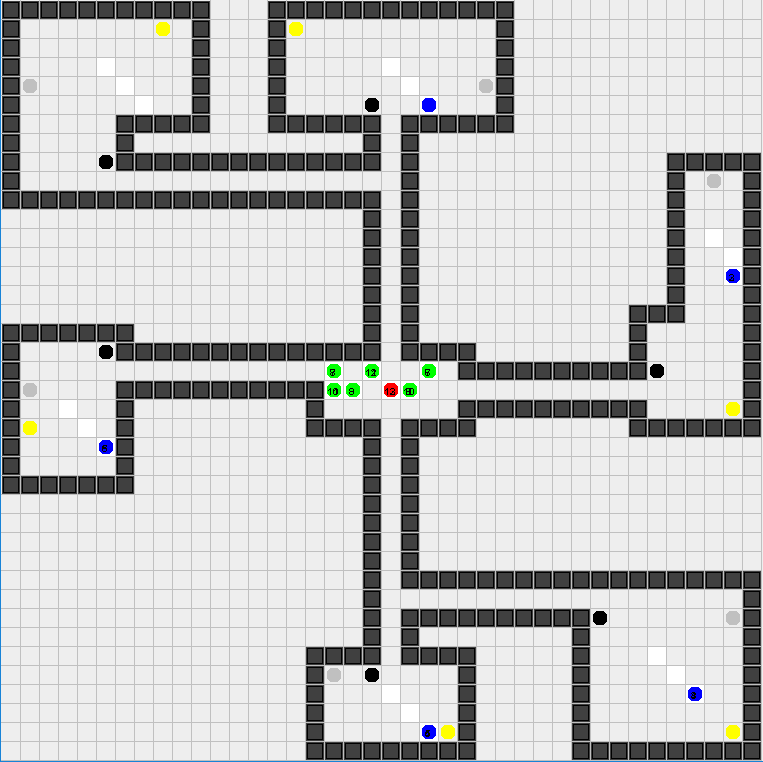
\includegraphics[scale = 0.55]{img/miniera.png}
  \caption{Rappresentazione della miniera}
\end{figure}
Il modello realizzato è formato da una griglia 50x50 che rappresenta una miniera composta da una serie di caverne.\\
Le sezioni nere del modello aiutano a rappresentare (anche visivamente) la sua struttura, delineando ostacoli non attraversabili dagli agenti del sistema.\\
La miniera è logicamente e fisicamente suddivisa dai seguenti elementi:
\begin{itemize}
	\item n.1 \textit{ControlCave}: posizionata al centro dell'intera miniera, è un punto focale di coordinamento per gli agenti.\\
	Ogni \textit{carrier}, infatti, ritornerà periodicamente all'interno di questa cave per ottenere dei compiti da svolgere e/o risorse richieste dai miners (ad esempio, birra).\\Al suo interno risiede staticamente l'unico agente \textit{forger} presente, rappresentato in rosso.\\
	\item n.6 \textit{MineCave}: dimora di ogni \textit{miner} del sistema, è il luogo nel quale le risorse previste del sistema vengono posizionate per essere raccolte.\\ Possono essere di varia forma e, per ipotesi semplificatrice, hanno un unica uscita che porta alla \textit{ControlCave} attraverso una serie di tunnel.\\
	Come già premesso, ogni \textit{MineCave} contiene esclusivamente un \textit{miner} (rappresentato da un pallino di colore blu) e da una serie di punti di interesse, qui elencati:
	\begin{itemize}
		\item Una vena di oro (in giallo)
		\item Una vena di ferro (in grigio)
		\item uno punto di stoccaggio (in nero) delle risorse raccolte localmente
	\end{itemize}\vspace*{0.4cm}
	
	\item \textit{Tunnel}: ogni \textit{MineCave} e collegata alla \textit{ControlCave} attraverso una serie di cunicoli chiamati \textit{Tunnel}.\\ Possono esistere più \textit{Tunnel} consecutivi che conducono a una stessa caverna.\\ Gli unici agenti in grado di percorrerli sono i \textit{carrier}, rappresentati in verde.
\end{itemize}
Ogni tipologia di caverna è una specializzazione della classe astratta \textit{Cave}, ognuna caratterizzata da una lista di oggetti \textit{Area} e un dizionario degli items contenuti:
\lstinputlisting[float=h,caption=Cave.java]{code/Cave.java}
\lstinputlisting[float=h,caption=MineCave.java]{code/MineCave.java}
\lstinputlisting[float=h,caption=ControlCave.java]{code/ControlCave.java}
%===========================================================================
%===========================================================================
\newpage

L'ambiente stesso presenta una serie di eventi stocastici che possono cambiare la behaviour degli agenti all'interno della società: ad esempio, ogni dieci secondi esiste il 33\% di probabilità che un orda di orchi minacci la miniera.\\
In tal caso, tutti gli agenti reagiranno a tali eventi in base a delle precise direttive: nel suddetto esempio il \textit{forger} inizierà a produrre armature (sempre ammesso che ci siano abbastanza risorse in magazzino), i \textit{miners}scaveranno soltanto ferro e i \textit{carriers} si interesseranno soltanto di prelevarlo dai magazzini locali delle \textit{MineCaves}.
\newpage
\subsection{Key aspects for Autonomous system}
%===========================================================================
%===========================================================================
\newpage
\section{Requirement analysis}
\labelsec{ReqAnalysis}
\subsection{(Domain)model}
The definition of a Domain model its used by software developers to express and describe the entities of the know system, in the form of structure, interaction and behaviour:\\\\
\textit{\textbf{Rover}}
\begin{itemize}
\item \textit{Structure:} a reactive and hardware-composed entity by a sonar and a motor.
\item \textit{Interaction:} can be controlled and interacted entirely with a series of commands and events, coming both from the final user and 										its sensors.
\item \textit{Behaviour:} consist in travelling trough a path between a point A and a point B.
During the route, it's capable of react accordingly to a series of events and user input.
\end{itemize}
%FIXME: inserire diagramma di stato per tutti i behaviours?
%FIXME:capire se come nome (sonar subsystem) può andare bene!
\textit{\textbf{Sonar system}}
\begin{itemize}
\item \textit{Structure:} it can be considered a composed entity: the user requiments explicity express the need of 2 indipendent sonars.\\It can be considered a proactive entity.
\item \textit{Interaction:} the only interaction this entity performs is the emission of informations in the form of events: in fact, no explicit command can be sent to this entity.\\
It should be noted that the emitted events are explicity defined in the requiments.
\item \textit{Behaviour:} Each of the sonar composing this subsystem must emit an event whenever a Robot passes in front of it. 
\end{itemize}
%FIXME: Tutta la descrizione di console allo stato attuale va bene?
\textit{\textbf{Console}}
\begin{itemize}
\item \textit{Structure:} a proactive component that let the user interact with the system.\\ It's mainly composed of a set of predefined graphical elements.
\item \textit{Interaction:} the only interaction this component performs is towards the robot.\\Being proactive, the interaction it's obiviously one-way.
\item \textit{Behaviour:} this entity has the sole purpose to intercept and forward the user commands to the robot.
\end{itemize}
%===========================================================================
%===========================================================================
\subsection{Logic architecture}
\begin{figure}[htbp]
  \centering
   \includegraphics[scale = 0.6]{img/logica.png}
  \caption{Logic architecture}
\end{figure}
\newpage
%===========================================================================
\section{Progetto}
\labelsec{Progetto}
Il progetto è stato sviluppato tramite \textit{Jason}, un interprete basato versione estesa di Agent Speak.\\
Come tutti i linguaggi utilizzati per programmare agenti BDI, \textit{Jason} permette di descrivere Belief, Goals e Plans attraverso regole Prolog-Like, oltre a rendere possibile la definizione di piani pienamente compatibili con codice Java.\\
\newpage
\subsection{Structure}

\subsection{Interaction}
\newpage
%===========================================================================
\section{Implementation}
\labelsec{Implementation}
Thanks to the generation performed by the XText Tool, nearly all the code of this project has been written by the use of \textit{qa} models.\\
All the source code directly written by this team can be found in the \textit{src} folder of the project; the generated source code files, however, can be found in two separate folders: \textit{src-gen} and \textit{srcMore}.\\
As a result of careful engineering process of the functional requiments we were able to keep minimal the abstraction gap of the project: only a single java file (of about ~70 lines of source code) is mandatory for the step 2, by containing all the \textit{javaRun} used by the rover.\\\\
We then proceed by presenting a brief explanation of all methods contained in \textit{it.unibo.custom.path}:
\begin{itemize}
\item \textit{register} it's a method called by the QActor rover to track and keep history of every physical movement performed.\\
The movements tracking is made possible by the use of a \textit{Stack} of custom objects called \textit{Action}, each containing the movement name, its duration and timeout value.\\
\item \textit{startReverse} permits, as the name suggests, to start a reverse sequence of all the actions tracked by the \textit{register} method: every registered movement will be sent back (in the correct order) to the rover by the use of qactor messages.
\end{itemize}
It should be noted that the actual implementation of the reverse mechanism has the peculiarity of recording in a "mirror" way some of the input data movements: for istance, "left" movements are registered as "right" in the data stack and viceversa.
\newpage
\subsection{GUI Commands}
Some of the functional requiments explained in the subsection \hyperref[sec:Functional requiments]{4.3} premise the user direct interaction with the system (for example it's made clear that the reverse sequence it's expressely started, at any moment, by the user if it deems).\\
Since no indication was given by the functional requiments, we opted for a \\manual insertion of commands from the GUI input box, as shown in the image below:\\

\hspace{-1cm}
 \includegraphics[scale=0.4]{img/gui.jpg} 
A definition of the actual commands for the system was also necessary, along with the ability to parameterize the inputs.\\
Therefore, we provide a brief list of the accepted commands of the system, with a synthetic explanation of their required parameters and effects:

\begin{table}[ht]
\hspace{-1cm}
\begin{tabular}{|l|l|l|}
\hline
\textbf{Command}             & \textbf{Parameters}                                                                                                                                  & \textbf{Effect}                                                                                                                                          \\ \hline
\textit{connectToUnity(X)}   & \begin{tabular}[c]{@{}l@{}}X: a string rapresenting the IP address \\ of the unity environment to connect to\end{tabular}                            & \begin{tabular}[c]{@{}l@{}}This command links the robot system to \\ its unity representation\end{tabular}                                               \\ \hline
\textit{setStartDistance(X)} & \begin{tabular}[c]{@{}l@{}}X: an integer value rapresenting the \\ starting distance between the robot\\ initial position and the sonar\end{tabular} & \begin{tabular}[c]{@{}l@{}}This command can be used to accordingly\\ set the initial starting position of the\\ rover (relative to sonar1).\end{tabular} \\ \hline
\textit{startReverse}        & \multicolumn{1}{c|}{/}                                                                                                                               & \begin{tabular}[c]{@{}l@{}}This command starts the reverse sequence\\ of the robot.\end{tabular}                                                         \\ \hline
\end{tabular}
\caption{Enabled commands from the GUI}
\end{table}
\newpage
%===========================================================================

%===========================================================================
\section{Testing}
\labelsec{testing}
Thanks to the unity game engine, virtualization of a real robot has been particularly useful: this way, all the problematics of a real world robot (circuitry, voltage regulation, motors calibration etc.) has been avoided, and so all the tests related to these hardware components.\\
Moreover, the unity scene let us to replicate instantly the environment the rover has to run across: this ease of use permitted the execution of a high number of stress tests with minimal effort.\\\\
Then, the behaviour of every single \textit{QActor} has been tested by forging a series of messages (or events, depending on the entity) and studying the consequent reaction.\\
This kind of tests has been part of our \textit{unit testing} plan described in section \hyperref[sec:Test plan]{5.4}.\\\\
Ensured that every single entity, taken individually, behave as expected, we then proceed to test the system in a whole; to our surprise, the integration of the different \textit{QActors} of the project lead to many issues and unexpected behaviour (more than the issues found during the previous testing phase), primarly due to calibration, timing and message exchange problems.\\
However, as stated above, the ease of use of the unity scene let us to perform an high number of integration tests in a reduced time window.\\\\
Finally, our concern has been to test the system in different network conditions: considering that it's possible for the user to connect to a remote unity scene (situated, for istance, in a different machine) we promptly tested this use case and also with a slow-network condition.
%===========================================================================

%===========================================================================
\section{Deployment}
\labelsec{Deployment}
The system will be deployed through a generated zip file by the gradle tool, which has the benefit of dealing and resolving all the necessary dependency of the project.\\
Fortunately, the configuration file for gradle is automatically generated by the XText tool on each iteration, granting an enormous simplification of this phase for each subsequent version; this could be also usefult to reduce the effort needed to train new developers on the development of the software.

%===========================================================================

%===========================================================================
\section{Maintenance}
\labelsec{Maintenance}
The system it's, on overall, greatly expandable and reusable: for example, the obstacles length, position, number and shape may vary with little to none necessary modifications to the source code.\\
In fact, our code ingegnerization should limit the changes needed for a non-trivial functional requirement to the sole \textit{rovermind} QActor, and leave the other parts of the project intact.

%Our system has been tested and validated so its components can be reused for future problems that involve differential drive robots, leds, distance sensors, WebCams. The custom language QActor is a solid meta-model that can be used to model any other distributed software system; QRobot and Baseddr are solid meta-models useful to model systems that include physical robots. A possible extension of the system is the installation of a real WebCam on the robot to capture photos of the surrounding environmen

%The system, as previously said and described, has been tested in each of its parts and it is functioning; moreover, the single parts can be used to create dierent kind of systems, realizing dierent behaviours. A possible, future extension could concern the adding of a WebCam on the Raspberry.

%The system is easily expandable and reusable. The configuration of the system is extremely simple with the introduction of Prolog rules and Java methods containing the variable system’s parameters. The choices made guarantee also strong flexibility even with new or modified requirements: for example, adding new sensors do not involve drastic changes to the system
%===========================================================================
\newpage

\bibliographystyle{abbrv}
\bibliography{biblio}

\end{document}

%RELAZIONE (domande e concetti)
premessa da piaga: chiedo scusa, alla fine di ogni capitolo nei commenti,
aggiungo dei concetti di teoria per comodità e per orientarci sul cosa scrivere nella relazione


1)INTRODUZIONE
Scopo della relazione
Introduzione a metodologie usate per sviluppare il progetto
Scopo dell'elaborato

2)VISIONE (si faccia riferimento soprattutto alla visione del percorso di riferimento)
Concetti e punti di vista sulle metodologie usate
Concetto teorico su cui si basa lo sviluppo del sistema software
Perchè è necessaria l'analisi?
Quali metodologie e modelli si possono sfruttare?
Perchè non UML?
Quale modello si può usare per creare il codice autogenerato?
Definire gli step del processo di produzione

Un percorso di riferimento:
L’artefatto relativo alla visione può essere un documento
che descrive le motivazioni generali che hanno indotto
una persona,gruppo, azienda a impegnarsi nello sviluppo dell’applicazione,
evidenziandone i benefici che provengono da essa.
L’artefatto relativo agli obiettivi è un documento che illustra gli obiettivi
che si vogliono raggiungere grazie allo sviluppo dell’applicazione o al suo uso
o sviluppi futuri. 
Insieme agli obiettivi è possibile legare un modello di business,
per esprimere il contesto dove il sistema opera e per definire un
vocabolario di termini utili alla fase di analisi dei requisiti.

Commento by piaga:
é possibile scrivere la relazione mantenendo la terza persona?
Secondo i concetti della vision scrivere "the usage of SCRUM framework for the dev...has perfectly satisfied..." potrebbe non essere corretto perchè lo fa sembrare un parere sulla conclusione del progetto
rispetto ad una possibile visione sul modo di procedere.
IMHO consiglierei scrivere qualcosa tipo:

Scrum è un framework per lo sviluppo..bla bla bla (primissimi concetti di teoria)
Scrum può essere utile nello sviluppo del progetto (intenzioni)
Queste due frasi le metterei alla fine e non all'inizio...
prima scriverei molto sulla visione generale del progetto.
Non so se è giusto ma scriverei qualcosa tipo:
"(ambiente attuale)Nel mondo dell'informatizzazione e dell'automazione, sempre più professioni scompariranno... 
(previsione)...è giusto quindi prevedere la necessità di automatizzare anche la mobilità di un drone.
(benefici del progetto) l'intenzione è quello di minimizzare l'intervento umano sull'autonomia di lavoro del drone"





3)GOAL
Definire gli obiettivi di progetto e in che modo s'intende procedere.

4)REQUISITI
Scrivere i requisiti (copiare di pari passo ai requisiti del prof !?)

5)ANALISI DEI REQUISITI
Definire il glossario
Definire i casi d'uso
Definire il dominio-modello

Commento by piaga:
RICHIAMI TEORIA
Si ricorda che la definizione di un sistema software implica spesso la definizione di una collezione di domini e di dipendenze tra domini. Il termine dominio descrive un mondo relativamente autonomo, reale o astratto,  costituito da un insieme di entità che operano in accordo a precise regole, politiche e vincoli. Le categorie di domini più usate sono:
Dominio di applicazione: è il sistema visto dall’utente
Dominio di architettura: sono le strategie globali del progetto
Dominio di servizio: fornisce servizi generici di supporto al dominio applicativo
Dominio di implementazione: sono le componenti o piattaforme software pre-esistenti o legacy.
Un dominio si rappresenta in UML da un package. Un dominio può fare assunzioni sulla esistenza di altri domini, caratterizzati da precise proprietà.
Visione
Requisiti
Analisi
Piano di collaudo
Piano di lavoro
Progetto
Implementazione
Collaudo
Deployment
Maintenance


ANALISI DEL PROBLEMA
Definire la metodologia con cui si effettua l'analisi del problema
Illustrare il problema di mantenere un buon livello di astrazione; da che piattaforma si parte, che linguaggio, in che modo si astrae? (fare riferimento alle relazioni)
Descrivere l'architettura logica
Descrivere il piano di testing

PIANO DI LAVORO
Come si vuole affrontare il problema dell'astrazione?
Quali sono i tempi e costi di lavoro?

PROGETTO IMPLEMENTAZIONE TESTING DEPLOYMENT MAINTENANCE
Guarda la relazione